% !TEX encoding = UTF-8 Unicode
%Präambel

%Report für große Doukumente. Dieser ist in Kapitel (\chapter{}) aufgeteilt
%\documentclass[12pt, a4paper, ngerman]{report} 

%Article für normale Doumente
\documentclass[12pt, a4paper, ngerman]{article}

%Deutsche Beschreibungen von generiertem Text (table of contents => Inhaltsverzeichnis)
\usepackage[ngerman]{babel}

%Umlaute
\usepackage[utf8]{inputenc}

%Schriftart Helvetica 
\usepackage[scaled]{helvet}

%Seitenränder
\usepackage{geometry}
%top = Abstand nach oben
%left = Abstand nach links
%right = Abstand nach rechts
%bottom= Abstand nach unten
%heapsep= Abstand zwische Kopfzeile und Text
%footskip= Abstand zwischen Text und Fußzeile
\geometry{a4paper, top=25mm, left=30mm, right=25mm, bottom=30mm, headsep=10mm, footskip=12mm}

%Farben nutzen
\usepackage{xcolor}

%Grafiken einbinden
\usepackage{graphicx}

%Zusätzliche Positionsbefehle
\usepackage{float} 

%Die Einrücktiefe bei einem neuen Absatz
\setlength{\parindent}{0pt}


%Fülltext
\usepackage{blindtext}

%Fuer Zitate	
\PassOptionsToPackage{backend=bibtex}{biblatex}
\usepackage[natbib=true,style=numeric]{biblatex}
\usepackage[babel,german=guillemets]{csquotes}
\bibliography{quellen.bib} 

% Aufnahme von \paragraph in das Inhaltsverzeichnis 
\setcounter{tocdepth}{4}  

%Nummerierung vertiefen, \paragraph kommt mit ins Inhaltsverzeichnis
\setcounter{secnumdepth}{4} 


%Eigene Kommandos
% Osi Modell
\newcommand{\osi}{ISO/OSI Referenzmodell\xspace}

%Ende Präambel
	
\begin{document}

\begin{titlepage}
		\begin{center}
			
\includegraphics[width=.8\linewidth]{Grafiken/logo_htw.jpg}\\[1cm]    
			\textsc{\LARGE Hochschule für Technik und Wirtschaft \newline Fakultät für Ingenieurwissenschaften}\\[1.5cm]
			\newcommand{\HRule}{\rule{\linewidth}{0.5mm}} \HRule \\[0.4cm] { \huge \bfseries Ausarbeitung Protokolle}\\[0.4cm]
			\HRule \\[1.5cm]

			\begin{minipage}{0.4\textwidth}
				\begin{flushleft} \large
					\emph{Autoren:}\\
					Deniz \\
					Christoph Drost 3576450
				\end{flushleft}
			\end{minipage}
			\hfill
			\begin{minipage}{0.4\textwidth}
				\begin{flushright} \large
					\emph{Betreuer:} \\
					Jonas Vogt, M.Sc.
				\end{flushright}
			\end{minipage}
			\vfill
			{\large \today}
		\end{center}
	\end{titlepage}


%Inhaltsverzeichnis auf eigener Seite
\tableofcontents
\newpage 

\section{Einleitung}
Im Folgenden sollen verschiedene Layer 2 Protokolle für kabelgebundene Netze miteinander verglichen werden. Um die Zusammenhänge besser erklären zu können, möchten wir erst auf das \osi eingehen.
\subsection{Das \osi}
\begin{figure}[h]
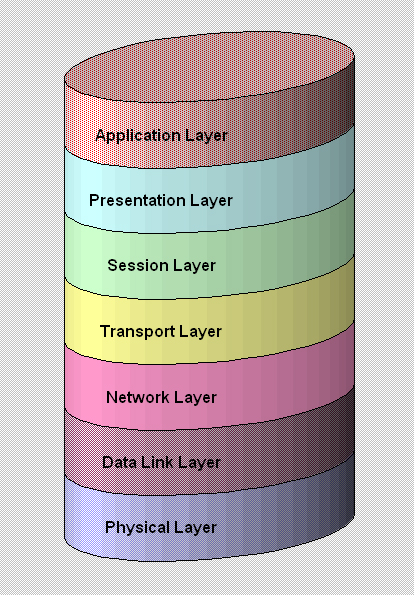
\includegraphics[width=0.5\textwidth]{Grafiken/osi_modell.jpg}
\caption{Das \osi im Überblick \cite{osi_modell}}
\label{osi_modell}
\end{figure} 
Diese Grafik stellt die Schichten des \osi da. Das \osi, (Open Systems Interconnection Model) ist ein allgemeines Kommunikationsmodell,  das die Kommunikation unterschiedlichster Geräte ermöglicht. Es beschreibt ein komplettes Telekommunikationsnetzwerk. Die einzelnen Funktionen sind in 7 Schichten aufgeteilt. 

Das \osi standardisiert die Netzwerk Architektur. Dadurch können Hersteller Lösungen anbieten, die auf der ganzen Welt genutzt werden können. Eine proprietäre Lösung hätte zu Insellösungen geführt. Ein weiterer Vorteil ist, dass die einzelnen Schichten, oder Layer, über Schnittstellen miteinander kommunizieren. Das ermöglicht ein Austauschen einzelner Komponenten, ohne die gesamte Architektur ändern zu müssen.

Da das \osi nur ein Referenzmodell darstellt, müssen die einzelnen Schichten konkret implementiert werden. Diese Implementierungen sind eigene Protokolle. 

\subsection{Der Layer 2}
Der Layer 2, Data Link Layer, setzt auf dem Physical Layer auf und stellt dem Network Layer seine Dienste zur Verfügung. Der Physical Layer beschriebt das Medium über das die Signale übertragen werden. Hier findet noch keine Logik statt. 

Die Aufgaben des Layer 2 im Überblick:
\begin{itemize}
	\item Aufteilung in Pakete
	\item Fehlerkontrolle
\end{itemize} 

\subsubsection{Aufteilung in Frames}
Die Datenblöcke werden im Layer 2 in Frames aufgeteilt. Die Vorteile des Framing sind die schnellere Nutzung eines shared Mediums und dass fehlerhafte Daten nicht komplett übertragen werden müssen.
\subsubsection{Fehlerkontrolle}
Der Data Link Layer führt eine Fehlerkontrolle durch. Dazu zählen eine Suche nach Duplikaten, nach inkorrekt oder unvollständig gesendeten Paketen. Wenn ein Fehler entdeckt wird, wird eine neue Übertragung der Frames angefordert \cite[S. 91]{SWB-107223570}. Die Fehlerkontrolle wird über den \glqq Cyclic Redundancy Check\grqq ~CRC durchgeführt. Dieses Verfahren ist eine Möglichkeit zur Prüfsummenberechnung, die beim Sender und der Senke durchgeführt wird. Sind beide Prüfsummen gleich, kann angenommen werden, dass das Frame korrekt übertragen wurde. 

Die Frames werden mit Sequence Numbers durchnummeriert. Der Empfänger prüft, ob die Frames in der richtigen Reihenfolge ankommen. Bei einer \glqq out-of-sequence transmission\grqq ~kann von einem verlorenen Frame ausgegangen werden, das entsprechende Frame wird neu angefordert, bzw. Layer 3 wird benachrichtigt.
\section{Die Layer 2 Protokolle im Überblick}

\subsection{Ethernet}
Ethernet ist ein weit verbreitetes Layer 2 Protokoll. 90\% aller lokal installierten Netzwerke sind mit Ethernet realisiert\cite{SWB-097965316}. Ethernet wurde ursprünglich für die Anbindung eines Druckers bei der Firma Xerox Corporation entwickelt. Die damalige Übertragungsgeschwindigkeit von 2,94 Mbit/s wurde auf aktuell 100 Gbit/s gesteigert, weitere Steigerungen sind zu erwarten.

Die Daten werden im Ethernet über einen eigenen Übertragungskanal transportiert. Kollisionen werden durch \glqq CSMA/CD\grqq ~entdeckt, bzw. aufgelöst. Die Übertragung läuft gleichberechtigt und verbindungslos. Die Daten werden an alle Teilnehmer weitergeleitet, diese vergleichen die Empfängeradresse mit ihrer eigenen und verwerfen die Frames, die nicht an sie adressiert sind. Diese Aussage kann eingeschränkt werden, da Switche die Daten nur an Ports leiten, an denen die entsprechenden Senken angeschlossen sind. 

\subsubsection{Gebräuchliche Übertragungsmedien des Ethernet}
\begin{figure}[H]
\begin{minipage}[hbt]{.28\linewidth}
	\centering
	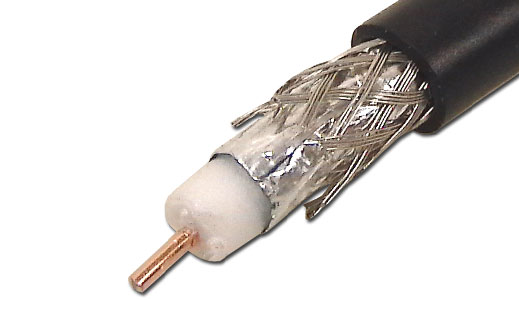
\includegraphics[width=0.9\linewidth]{Grafiken/koaxkabel.png}
	\caption{Koaxkabel \cite{koax_kabel}}
	\label{koaxkabel}
\end{minipage}
\hfill
\begin{minipage}[hbt]{.28\linewidth}
	\centering
	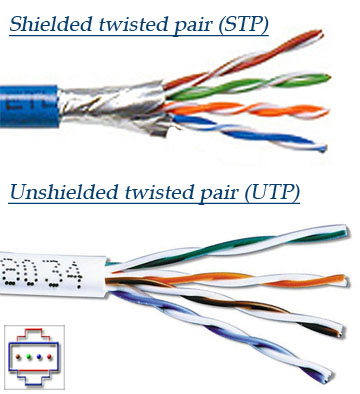
\includegraphics[width=0.9\linewidth]{Grafiken/twistetPair.jpg}
	\caption{Twistet Pair Kabel \cite{tw_kabel}}
	\label{twkabel}
\end{minipage}
\hfill
\begin{minipage}[hbt]{.28\linewidth}
	\centering
	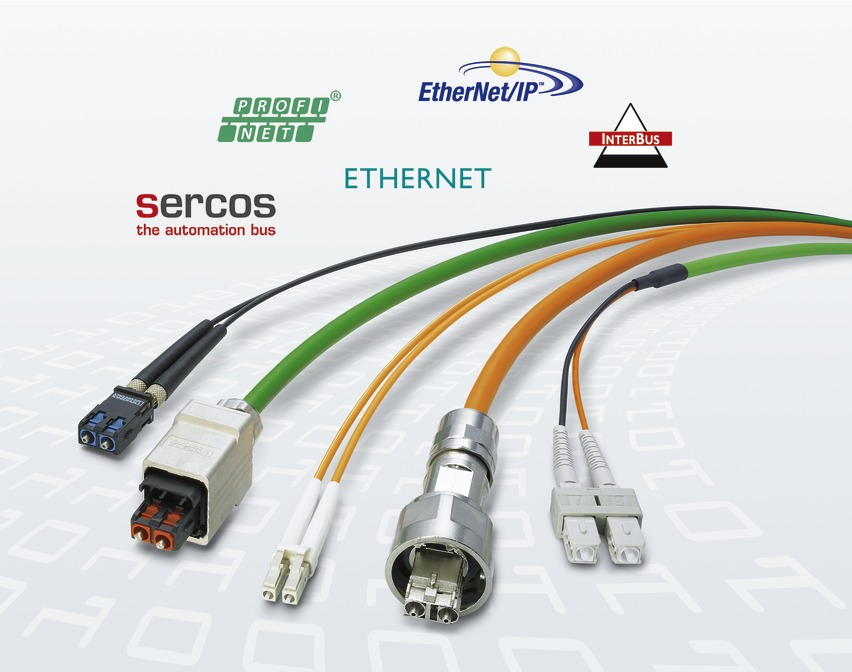
\includegraphics[width=0.9\linewidth]{Grafiken/lwl_leiter.jpg}
	\caption{Lichtwellenleiter \cite{lwl_leiter}}
	\label{lwlleiter}
\end{minipage}
\end{figure}
 
Historisch gesehen muss das Koaxialkabel als Medium des Ethernet genannt werden. Das Koaxkabel wurde 1990 mit der Einführung von 10BaseT (IEEE 802.3i) durch Unshielded Twisted Pair Kabel ersetzt. Ab 1998 wurden mit der Einführung des Gigabit Ethernet auch Lichtwellenleiter genutzt. 

\subsubsection{Adressierung}
 Ethernet nutzt zur Adressierung von Teilnehmern deren MAC-Adresse. MAC-Adressen, Media Access Control Adress, sind Hardwareadressen und werden weltweit eindeutig vergeben. Sie bestehen aus 6 Byte und sind nach folgendem Muster aufgebaut: 
 
 Hersteller--Hersteller--Hersteller--xx--xx--xx 

Der Herstellerteil, auch Organizationally  Unique Identifier (OUI), wird von der IEEE vergeben. Jeder Hersteller hat seinen eigenen Bereich, der durch die ersten 3 Bytes bestimmt wird. Die letzten 3 Bytes werden vom Hersteller selber vergeben. Dabei ist der Hersteller für die eindeutige Vergabe der letzten 3 Bytes verantwortlich. Einige Hersteller haben mittlerweile mehrere eigene Bereiche.

\subsubsection{Zugriff auf das Medium}
Historisch gesehen nutzt Ethernet das Übertragungsmedium als Shared Medium. Die einzelnen Teilnehmer wurden am selben Koaxialkabel über T-Stücke angeschlossen. Um Kollisionen zu vermeiden, wurde ein geeignetes Verfahren zur Vermeidung benötigt. Von einer Kollision spricht man, wenn mehrere Teilnehmer gleichzeitig auf das Medium zugreifen würden, also Signale aussenden. Die Signale würden sich gegenseitig überlagern und wären nicht mehr nutzbar. Bei Ethernet wird CSMA/CD eingesetzt. Bei diesem Verfahren wird vor dem Senden geprüft, ob die Leitung frei ist. Erst wenn die Leitung frei ist wird gesendet (Carrier Sense). Wenn zufällig mehrere Teilnehmer gleichzeitig ein Signal aussenden (Multiple Access) kommt es dennoch zu Kollisionen. Der/Die Sender prüfen während dem Senden, ob es zu Kollisionen kommt (Collision Detect) und brechen ihre Übertragung im Fall einer Kollision ab. Nach einem Abbruch wird eine zufällige Zeit gewartet bis erneut gesendet wird.

Historisch gesehen nutzt Ethernet das Übertragungsmedium als Shared Medium. Die einzelnen Teilnehmer wurden am selben Koaxialkabel über T-Stücke angeschlossen. Um Kollisionen zu vermeiden, wurde ein geeignetes Verfahren zur Vermeidung benötigt. Von einer Kollision spricht man, wenn mehrere Teilnehmer gleichzeitig auf das Medium zugreifen würden, also Signale aussenden. Die Signale würden sich gegenseitig überlagern und wären nicht mehr nutzbar. Bei Ethernet wird CSMA/CD eingesetzt. Bei diesem Verfahren wird vor dem Senden geprüft, ob die Leitung frei ist. Erst wenn die Leitung frei ist wird gesendet (Carrier Sense). Wenn zufällig mehrere Teilnehmer gleichzeitig ein Signal aussenden (Multiple Access) kommt es dennoch zu Kollisionen. Der/Die Sender prüfen während dem Senden, ob es zu Kollisionen kommt (Collision Detect) und brechen ihre Übertragung im Fall einer Kollision ab. Nach einem Abbruch wird eine zufällige Zeit gewartet bis erneut gesendet wird. Der Grund, warum es trotz diesem Verfahren zu Kollisionen kommen kann, ist die Signallaufzeit. Die Signale brauchen eine gewisse Zeit um über die Leitungen übertragen zu werden. 

In seinen Anfangszeiten übertrug Ethernet im Halbduplex Verfahren. Das bedeutet, dass ein Übertragungskanal zum Senden und zum Empfangen genutzt wird. Dadurch halbiert sich natürlich im schlimmsten Fall die Datenrate. Mit der Einführung von Twisted Pair Kabeln und Lichwellenleitern wurde Ethernet auf den Vollduplex Betrieb umgestellt. Dadurch konnte die Übertragungsrate gesteigert werden und Kollisionen wurden unwahrscheinlicher.
\begin{figure}[H]
	\centering
	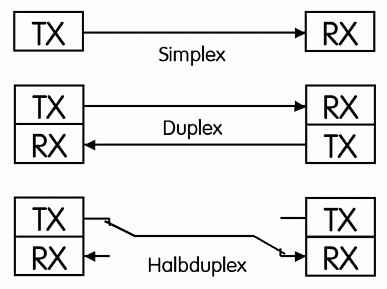
\includegraphics[width=0.4\linewidth]{Grafiken/duplex.jpg}
	\caption{Unterschied der Duplex Übertragungen \cite{duplex}}
	\label{duplex}
\end{figure}
 
 \subsubsection{Frames}
Um Daten über Ethernet übertragen zu können werden sie in Frames aufgeteilt. Der Vorteil daran ist, dass ein Sender bei großen Übertragungen nicht das gesamte Netzwerk belegt und dass bei einer fehlerhaften Übertragung nur einzelne Frames neu versandt werden müssen. Der Ausdruck Frame kann wörtlich genommen werden. Die Nutzdaten werden in einen Rahmen (Frame) eingepackt.

Neben den eigentlichen Nutzdaten enthält ein Frame:
\begin{itemize}
	\item Die Präambel (dient u.a. zur Synchronisation der Empfängerstationen) 
	\item Die Hardware Quell- und Zieladresse
	\item Ein Typ- oder Längenfeld
	\item Eine Checksumme
\end{itemize}
\begin{figure}[H]
	\centering
	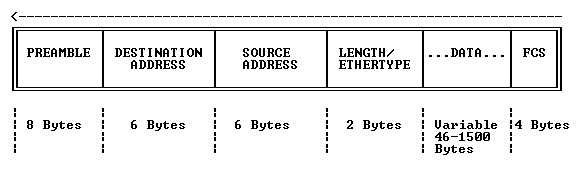
\includegraphics[width=0.9\linewidth]{Grafiken/ethernet_frame.jpg}
	\caption{Ethernet 802.3 Frame \cite{ethernet_frame}}
	\label{ethernet_frame}
\end{figure}

Die Präambel enthält eine Bitfolge, die dem Empfänger signalisiert, dass ein Rahmen ankommt. Die Präambel besteht aus 8 Bytes mit einer alternierenden Folge aus 0 und 1. Die letzten 2 Bits im letzten Byte sind immer 1. Hier besteht ein kleiner Unterschied zwischen DIX und IEEE. Obwohl die Bitfolgen die gleichen sind, ist die Präambel im IEEE Standard formell in die 7 Byte lange Präambel und den 1 Byte langen Start-of-Frame-Delimiter aufgeteilt.
 
Die Adressen sind MAC Adressen. Dieser werden von der IEEE an die Hersteller von Ethernet Komponenten vergeben und müssen weltweit eindeutig sein.

\subsubsection{Topologie}
Ethernet ist keiner bestimmten Netzwerk Topologie zuzuordnen. Heute gebräuchlich ist eine Sterntopologie, andere Formen sind aber auch möglich.   

\subsection{LAPD}
LAPD, Link Access Procedure on the D-channel ist auch ein Protokoll der Schicht 2. Es wird genutzt um Layer 3 Informationen zwischen den Teilnehmer des ISDN Netzwerks zu übertragen. Für diese Übertragung wird der D-Kanal genutzt.

\subsubsection{Der D-Kanal}
Der D-Kanal wird im ISDN zur Signalisierung genutzt. Er stellt 16 kbit/s zur Verfügung. Signalisieren bedeutet, dass der Teilnehmer und die Vermittlungsanlage Informationen austauschen. Das können Informationen sein, ob der Teilnehmer verfügbar ist, oder auch Informationen mit denen ein Gespräch aufgebaut wird. Im Gegensatz zu den B-Kanälen, über die Nutzdaten, wie z.B. Sprache, übertragen wird, kommunizieren über den D-Kanal nur Prozessoren.

\subsubsection{Adressierung \label{tei}}
LAPD nutzt zur Adressierung der Teilnehmer den TEI, Terminal Endpoint Identifier. Der TEI wird entweder durch eine feste Einstellung im Endgerät oder durch die Vergabe der Vermittlungsstelle vergeben. Er besteht aus 7 Bit. Der TEI ist im normalen Betriebszustand eindeutig, darf aber nicht mit der Rufnummer verwechselt werden.

\subsubsection{Frames}
LAPD teilt die Daten der Schicht 3 in Frames auf. Dabei werden unterschiedliche Frametypen benutzt. Ein Frame ist ist folgendermaßen aufgebaut:

\begin{itemize}
	\item Blockbegrenzung
	\item Adressfeld
	\item Steuerfeld
	\item Daten
	\item Blockprüfung
	\item Blockbegrenzung
\end{itemize}

\begin{figure}[H]
	\centering
	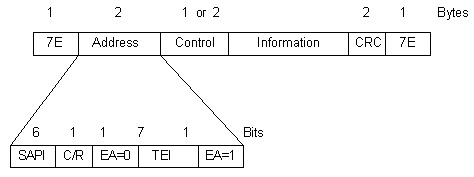
\includegraphics[width=0.9\linewidth]{Grafiken/lapd_frame.jpg}
	\caption{LAPD Frame \cite{lapd_rahmen}}
	\label{lapd_frame}
\end{figure}

\paragraph{Blockbegrenzung}
Die Blockbegrenzung ist eine Byte, das aus eine Bitkombination besteht, die im restlichen Block nicht vorkommt. Sie stellt den Anfang und das Ende des Blocks dar. \textcolor{red}{\textbf{Sollen wir das noch genauer ausführen?}}  S.448 Technik der Netze.  

\paragraph{Adressfeld}
Das Adressfeld besteht aus 2 Bytes. Es enthält den SAPI und den TEI, die je 1 Byte groß sind. Die Größe 1 Byte ist eigentlich ungenau, da man die Bytes wieder genauer aufteilen kann. Jedes dieses Bytes hat ein EA (Extended Adress), damit wird angegeben, ob dem Byte noch weitere folgen. Der SAPI, Service Access Point Identifier,  identifiziert die Dienste der Schicht 2. Er besteht aus 6 Bit, zusätzlich sind in dem Byte das C/R Bit und das EA Bit. Das C/R-Feld kennzeichnet, ob das Paket eine Anweisung (Command) für den Empfänger enthält oder ob es eine Antwort (Response) auf eine zuvor erhaltene Anweisung enthält. 

Aktuell sind 3 Typen des SAPI definiert \cite{SWB-098672061}. 
\begin{itemize}
	\item Die gesicherte Übermittlung von Signalisierungsinformationen (SAPI 0)
	\item Die Übertragung von paketvermittelteten Daten (SAPI 16)
	\item Die Festlegung von eindeutigen TEI (SAPI 63)
\end{itemize}



Der TEI wurde bereits in~\ref{tei} genauer beschrieben. Im Byte des TEI wird EA = 1 gesetzt, da der TEI das letzte Adress Byte ist.

\paragraph{Steuerfeld}
Das Steuerfeld gibt an, 




\subsection{PPP}
Router - Router und Host - Netzwork Verbindungen über synchrone und asynchrone Kreise. Enthält ein Protokoll Feld um das Network Layer Protokoll zu Identifizieren \cite[S. 102]{SWB-107223570}  

\section{Bedeutungen der Protokolle im \osi }

%indirekte Quellen einbinden
\nocite{*} 

%Quellenangabe auf eigener Seite
\newpage
\sloppy
\printbibliography 



%Abbildungsverzeichnis auf eigener Seite
\newpage
\listoffigures

\end{document}